\documentclass{standalone}
% translate with >> pdflatex -shell-escape <file>

% This file is an extract of the PGFPLOTS manual, copyright by Christian Feuersaenger.
% 
% Feel free to use it as long as you cite the pgfplots manual properly.
%
% See
%   http://pgfplots.sourceforge.net/pgfplots.pdf
% for the complete manual.
%
% Any required input files (for <plot table> or <plot file> or the table package) can be downloaded
% at
% http://www.ctan.org/tex-archive/graphics/pgf/contrib/pgfplots/doc/latex/
% and
% http://www.ctan.org/tex-archive/graphics/pgf/contrib/pgfplots/doc/latex/plotdata/

\usepackage{pgfplots}
\pgfplotsset{compat=newest}

\pagestyle{empty}

\begin{document}
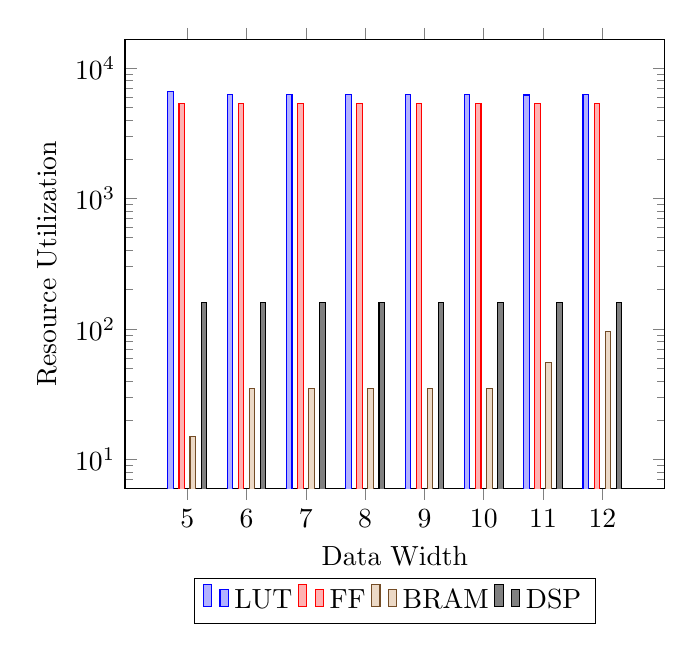
\begin{tikzpicture}
\begin{semilogyaxis}[
    ybar,
    enlargelimits=0.15,
    legend style={at={(0.5,-0.20)},
      anchor=north,legend columns=-1},
    ylabel={Resource Utilization},
    xlabel={Data Width},
    symbolic x coords={5,6,7,8,9,10,11,12},
    xtick=data,
    %nodes near coords,
    %nodes near coords align={horizontal},
    bar width=2pt,
    ]
\addplot coordinates {(5,6597) (6,6224) (7,6222) (8,6223) (9,6222) (10,6210) (11,6204) (12,6270)};
\addplot coordinates {(5,5368) (6,5303) (7,5303) (8,5303) (9,5303) (10,5303) (11,5303) (12,5303)};
\addplot coordinates {(5,15) (6,35) (7,35) (8,35) (9,35) (10,35) (11,55) (12,95)};
\addplot coordinates {(5,160) (6,160) (7,160) (8,160) (9,160) (10,160) (11,160) (12,160)};
\legend{LUT,FF,BRAM,DSP}
\end{semilogyaxis}
\end{tikzpicture}
\end{document}